\documentclass[11pt,a4paper]{ctexart}
\usepackage{geometry}
\geometry{margin=2.2cm}
\usepackage{graphicx}
\usepackage{tabularx}
\usepackage{booktabs}
\usepackage{array}
\usepackage{xcolor}
\usepackage{caption}
\usepackage{enumitem}
\definecolor{paper}{HTML}{F6F1E7}
\definecolor{ink}{HTML}{2B2622}
\definecolor{brandred}{HTML}{B3261E}
\definecolor{linkred}{HTML}{8A2318}
\definecolor{linkblue}{HTML}{5B7D99}
\usepackage{hyperref}
\hypersetup{colorlinks=true,linkcolor=linkred,urlcolor=linkblue,citecolor=linkblue}
\renewcommand{\arraystretch}{1.25}
\captionsetup{font=small,labelfont={bf,color=brandred}}
\setlist{itemsep=2pt,topsep=3pt}

\title{\textbf{AUTHEN 消费者端鉴真系统\\140 条真实算法/API 批测报告}}
\author{QA-140 合并复算与首页变更证据包}
\date{2026 年 10 月 20 日}

\begin{document}
\maketitle
\thispagestyle{empty}

\begin{abstract}
\noindent\textbf{结论先行：}本报告合并 shard\_01（前 70 条）与 shard\_02（后 70 条）两份真实批测明细，共 \textbf{140 条}，全部实际发出 HTTP 请求并留存原始请求/响应。\textbf{140 条 HTTP 状态均为 200，但 HTTP 200 不等于通过}；按「APP 实际五类判定与参考标签五类完全一致」的严格口径复算，\textbf{严格通过 17 条，未通过 123 条，严格通过率 12.14\%}。本批为\textbf{算法/API 流程批测}，浏览器 RPA 仅对首页三张场景卡做一次性冒烟，不参与 140 条结果；本批只验证现有规则/API 是否正确执行，\textbf{专业鉴伪能力（AI 生成检测、视频逐帧篡改、音频合成鉴定、专业功效核验）尚未全部接入，未在本批验证}。
\end{abstract}

\tableofcontents
\newpage

% ===================== 1 =====================
\section{测试范围与数据口径}

\subsection{被测对象与调用入口}
被测对象为本地消费者端网页 APP（源码 \texttt{AUTHEN/web/}，企业端未启用、未改动）。140 条全部真实调用同源服务端 \texttt{web/server.mjs} 的 \texttt{POST /api/review}（pipeline \texttt{inspect}，multi-agent-6dim-v2）；音频/视频先经同实例 \texttt{POST /api/transcribe}（faster-whisper small）转写再送鉴真。shard\_01 实例端口 4191，shard\_02 实例端口 4192，均为本地独立进程。

\subsection{数据包与参考标签}
- 数据包：\texttt{AUTHEN\_多模态测试数据包\_v2\_140条}（构造/脱敏验收集，\texttt{manifest\_labels.jsonl} 共 140 条参考标签）。
- 参考标签为\textbf{构造样本的人工标注，非第三方真值}，结果不得表述为真实平台准确率；答案（annotations、manifest\_labels）未进入任何模型请求。
- 合并时已用 \texttt{manifest\_labels.jsonl} 对每条记录的期望判定、模态、场景做独立交叉校验，0 条不一致。

\subsection{五类判定与严格通过定义}
APP 总判定限定五类：\textbf{暂未发现问题 / 有明确问题 / 线索级（待核验）/ 资料不足 / 无法判定}。

\begin{itemize}
\item \textbf{严格通过}：APP 实际五类判定 == 参考标签期望五类，逐字完全一致。
\item \textbf{HTTP 200 / API 成功只表示流程跑通}（服务在线、请求被解析、返回 JSON），\textbf{不得计为通过}；本批 140 条全部 200，与通过数 17 条形成明确对照。
\item error\_type：\texttt{none}（一致）/ \texttt{verdict\_mismatch}（五类不一致）；本批无 http\_error、pipeline\_failed、transport\_error。
\item mismatch\_kind：\texttt{missed\_conflict}（漏报明确问题）、\texttt{false\_alarm\_or\_clue}（干净样本误报/提前给线索）、\texttt{other}（其他不一致）。
\end{itemize}

\subsection{批测与冒烟的边界（重要）}
\begin{itemize}
\item 140 条均为\textbf{算法/API 批测}：脚本按前端真实提交格式构造请求，逐条发送并落盘原始请求/响应/日志。
\item \textbf{浏览器 RPA 只对首页三张场景卡（种草内容 / 评论区 / 图片视频音频）做一次性冒烟}，验证弹窗预选、引导条与选文件触发可用；RPA 结果不计入 140 条通过统计。
\item 本批区分「现有规则/API 是否正确执行」与「专业鉴伪能力是否验证」：后者尚未全部接入，不得据本批结果宣称具备专业鉴伪能力。
\end{itemize}

% ===================== 2 =====================
\section{总体结果}

\begin{figure}[h]
\centering
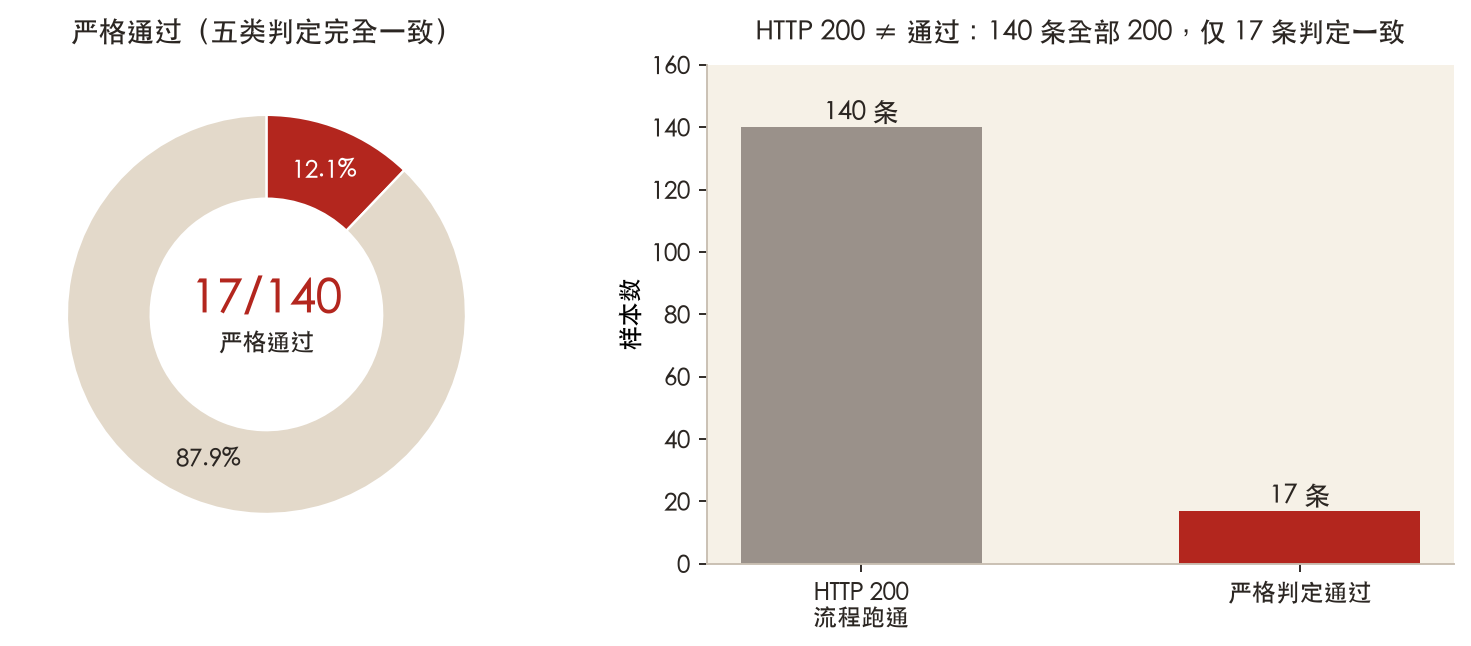
\includegraphics[width=0.92\textwidth]{../figures/fig1_pass_overview.png}
\caption{严格通过概览：140 条全部 HTTP 200，仅 17 条五类判定一致（12.14\%）}
\end{figure}

\begin{table}[h]
\centering
\small
\begin{tabularx}{\textwidth}{@{}lXXXX@{}}
\toprule
批次 & 样本数 & 严格通过 & 未通过 & 严格通过率 \\
\midrule
shard\_01（前 70：音频/评论/图文/文章/图片） & 70 & 13 & 57 & 18.57\% \\
shard\_02（后 70：图片/图文/文章/视频/转发变体） & 70 & 4 & 66 & 5.71\% \\
\textbf{合计} & \textbf{140} & \textbf{17} & \textbf{123} & \textbf{12.14\%} \\
\bottomrule
\end{tabularx}
\end{table}

\begin{table}[h]
\centering
\small
\begin{tabularx}{0.92\textwidth}{@{}lXX@{}}
\toprule
流程指标 & 数量 & 说明 \\
\midrule
HTTP 200 & 140 & 全部流程跑通，不等于判定通过 \\
verdict\_mismatch & 123 & 五类判定不一致 \\
none（一致） & 17 & 严格通过 \\
非 200 / 传输失败 / 流水线失败 & 0 & 无 \\
\bottomrule
\end{tabularx}
\end{table}

% ===================== 3 =====================
\section{期望判定与实际判定分布}

\begin{figure}[h]
\centering
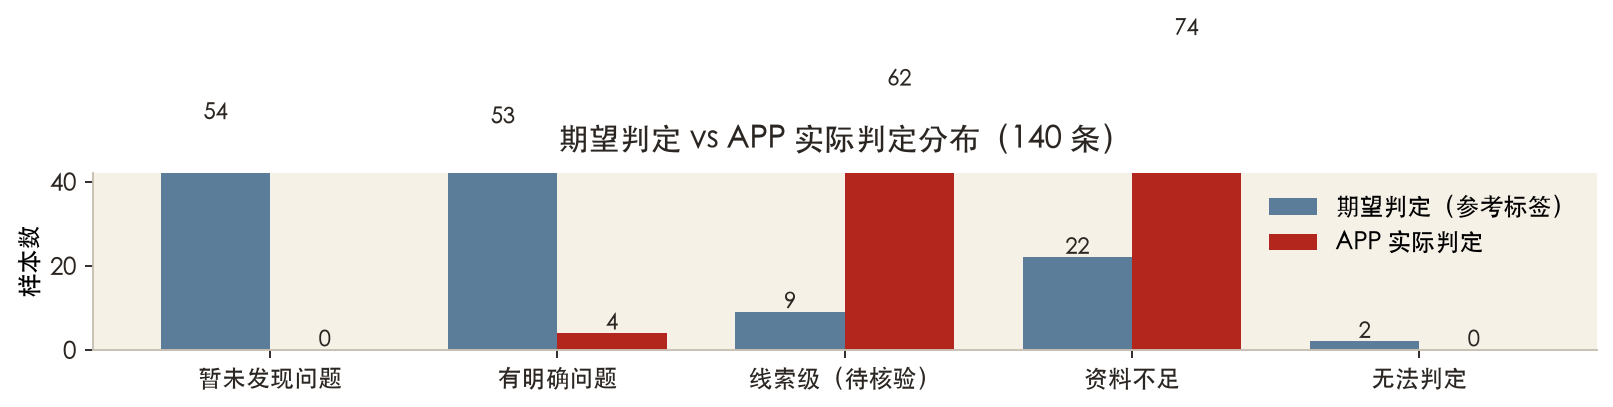
\includegraphics[width=0.92\textwidth]{../figures/fig2_expected_vs_actual.png}
\caption{期望判定（蓝）与 APP 实际判定（红）分布对比}
\end{figure}

\begin{table}[h]
\centering
\small
\begin{tabularx}{\textwidth}{@{}lXXX@{}}
\toprule
五类判定 & 期望分布 & 实际分布 & 差值（实际$-$期望） \\
\midrule
暂未发现问题 & 54 & 0 & $-54$ \\
有明确问题 & 53 & 4 & $-49$ \\
线索级（待核验） & 9 & 62 & $+53$ \\
资料不足 & 22 & 74 & $+52$ \\
无法判定 & 2 & 0 & $-2$ \\
\bottomrule
\end{tabularx}
\end{table}

\noindent\textbf{观察：}APP 实际输出高度集中在「线索级（待核验）62」与「资料不足 74」，未输出「暂未发现问题」与「无法判定」；对期望「有明确问题」与「暂未发现问题」的两端样本普遍向中间降级，呈现保守的「线索/资料不足」倾向。

% ===================== 4 =====================
\section{混淆矩阵：期望行 $\times$ 实际列}

\begin{figure}[h]
\centering
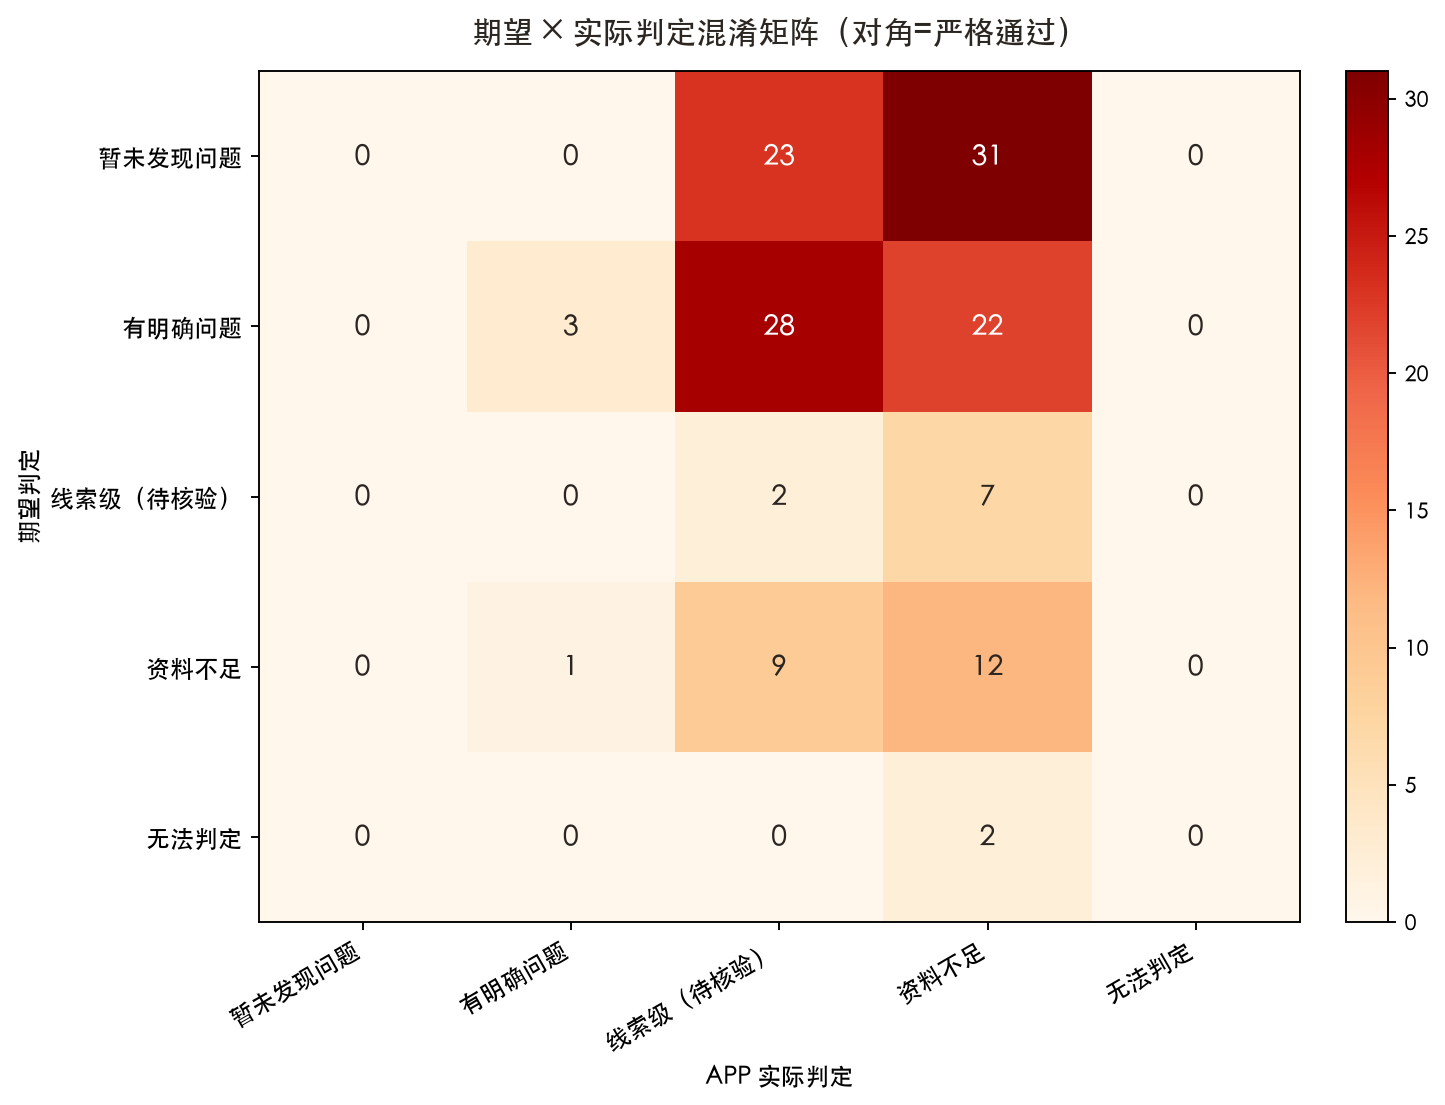
\includegraphics[width=0.86\textwidth]{../figures/fig5_confusion.png}
\caption{期望 $\times$ 实际判定混淆矩阵，对角元素之和为严格通过数 17}
\end{figure}

\begin{table}[h]
\centering
\footnotesize
\begin{tabularx}{\textwidth}{@{}lXXXXX@{}}
\toprule
期望 \textbackslash 实际 & 暂未发现问题 & 有明确问题 & 线索级 & 资料不足 & 无法判定 \\
\midrule
暂未发现问题 & 0 & 0 & 23 & 31 & 0 \\
有明确问题 & 0 & \textbf{3} & 28 & 22 & 0 \\
线索级（待核验） & 0 & 0 & \textbf{2} & 7 & 0 \\
资料不足 & 0 & 1 & 9 & \textbf{12} & 0 \\
无法判定 & 0 & 0 & 0 & 2 & 0 \\
\bottomrule
\end{tabularx}
\end{table}

\noindent 对角合计：$3+2+12=17$。主要错向：期望「暂未发现问题」54 条中 23 条被给线索、31 条判资料不足；期望「有明确问题」53 条中 28 条降级为线索、22 条降级为资料不足，仅 3 条命中。

% ===================== 5 =====================
\section{分模态统计}

\begin{figure}[h]
\centering
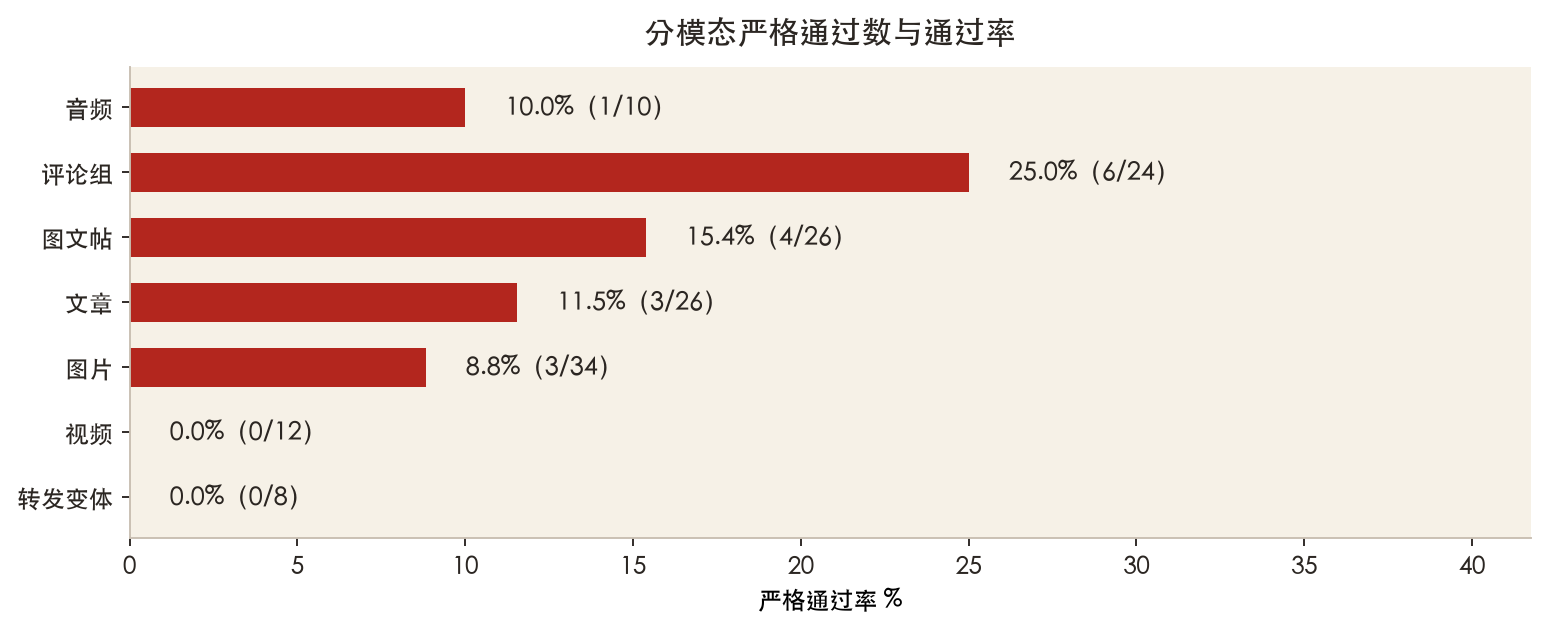
\includegraphics[width=0.9\textwidth]{../figures/fig3_modality.png}
\caption{分模态严格通过数与通过率（括号内为 通过/总数）}
\end{figure}

\begin{table}[h]
\centering
\small
\begin{tabularx}{\textwidth}{@{}lXXXX@{}}
\toprule
模态 & 样本数 & 严格通过 & 未通过 & 严格通过率 \\
\midrule
音频 & 10 & 1 & 9 & 10.0\% \\
评论组 & 24 & 6 & 18 & 25.0\% \\
图文帖 & 26 & 4 & 22 & 15.4\% \\
文章 & 26 & 3 & 23 & 11.5\% \\
图片 & 34 & 3 & 31 & 8.8\% \\
视频 & 12 & 0 & 12 & 0.0\% \\
转发变体 & 8 & 0 & 8 & 0.0\% \\
\bottomrule
\end{tabularx}
\end{table}

\noindent 评论组通过率最高（6/24，多为「资料不足」命中）；视频（12）与转发变体（8）零通过。需注意：多数「通过」集中在双方都判「资料不足」的保守情形，不等于鉴伪能力正确。

% ===================== 6 =====================
\section{分场景（split）统计}

\begin{figure}[h]
\centering
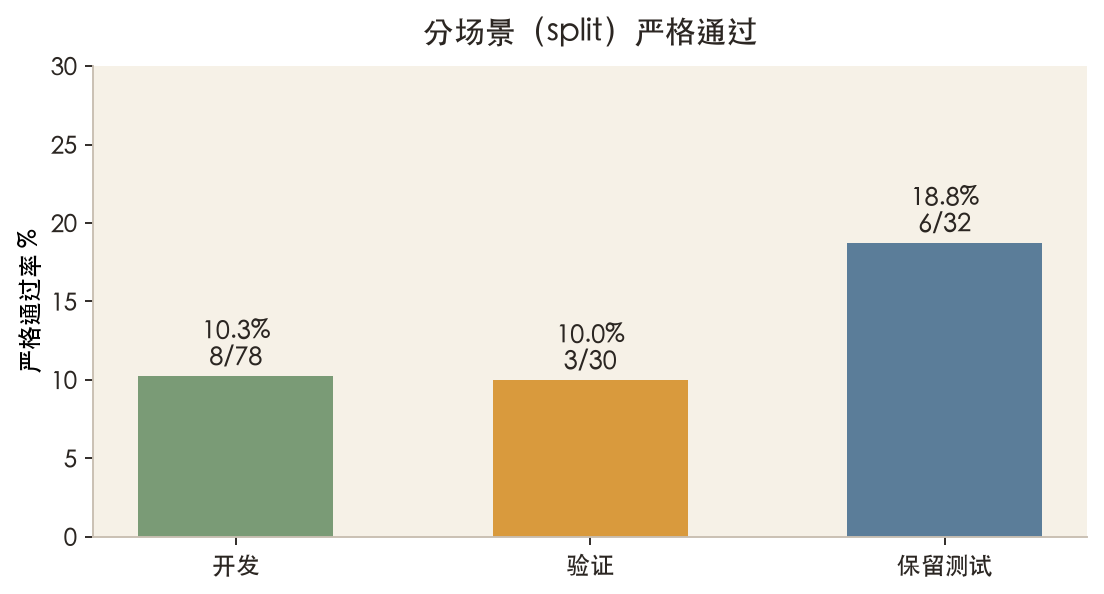
\includegraphics[width=0.62\textwidth]{../figures/fig4_scenario.png}
\caption{分场景严格通过}
\end{figure}

\begin{table}[h]
\centering
\small
\begin{tabularx}{0.8\textwidth}{@{}lXXX@{}}
\toprule
场景 & 样本数 & 严格通过 & 通过率 \\
\midrule
开发 & 78 & 8 & 10.26\% \\
验证 & 30 & 3 & 10.00\% \\
保留测试 & 32 & 6 & 18.75\% \\
\bottomrule
\end{tabularx}
\end{table}

% ===================== 7 =====================
\section{失败分布}

\begin{figure}[h]
\centering
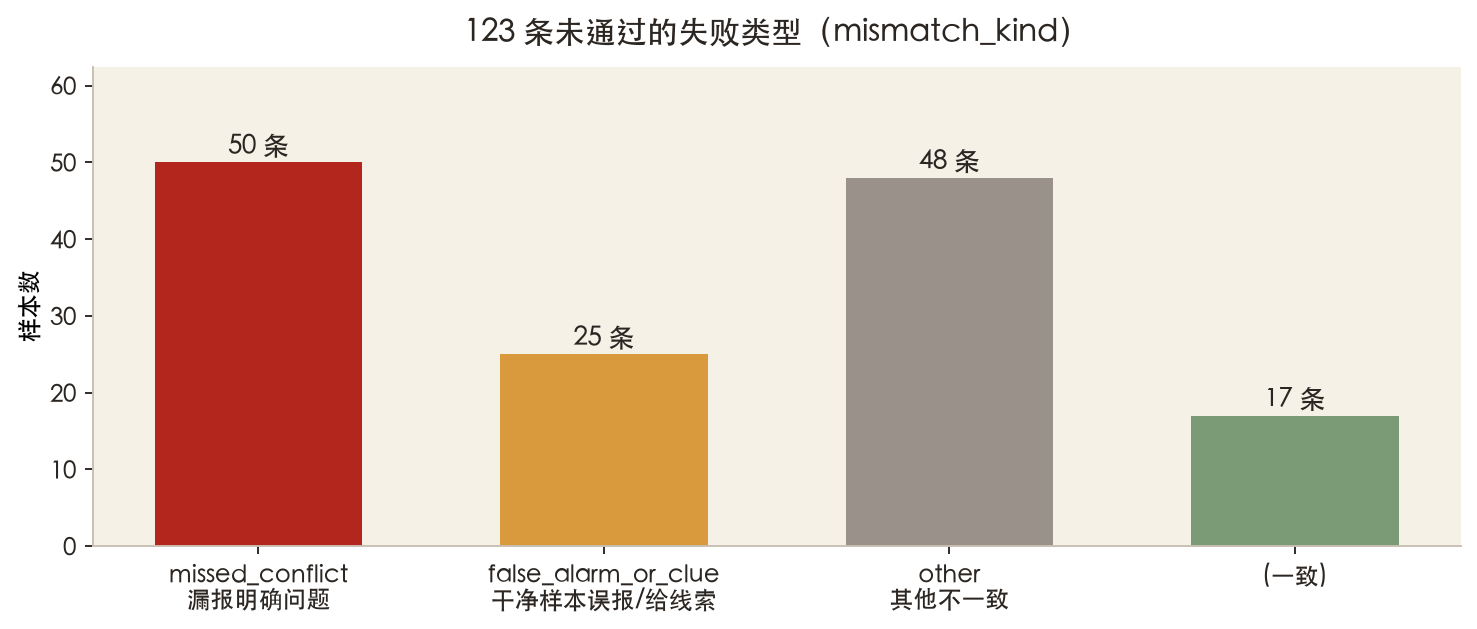
\includegraphics[width=0.9\textwidth]{../figures/fig6_mismatch.png}
\caption{123 条未通过的失败类型分布}
\end{figure}

\begin{table}[h]
\centering
\small
\begin{tabularx}{0.9\textwidth}{@{}lXX@{}}
\toprule
mismatch\_kind & 数量 & 含义 \\
\midrule
missed\_conflict（漏报明确问题） & 50 & 期望「有明确问题」被降级为线索/资料不足 \\
false\_alarm\_or\_clue（误报/给线索） & 25 & 干净或资料不足样本被提前给线索/明确问题 \\
other（其他不一致） & 48 & 其余类别错配（含资料不足$\leftrightarrow$线索等） \\
（一致，严格通过） & 17 & — \\
\bottomrule
\end{tabularx}
\end{table}

\begin{figure}[h]
\centering
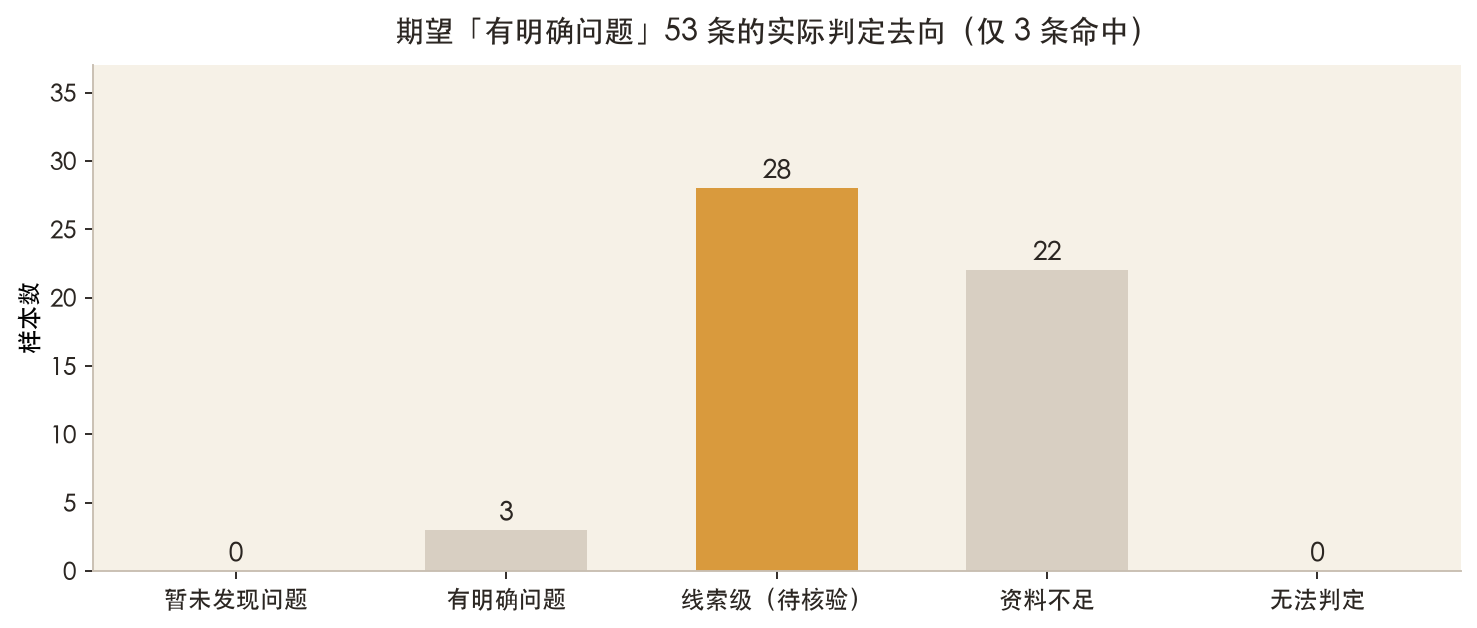
\includegraphics[width=0.9\textwidth]{../figures/fig7_missed_flow.png}
\caption{期望「有明确问题」53 条的实际去向：仅 3 条命中，28 条降级为线索、22 条降级为资料不足}
\end{figure}

\noindent 失败以\textbf{漏报为主}（50 条）：现有规则链倾向给「线索级/资料不足」，不敢落到「有明确问题」；其次为误报/提前给线索（25 条）。

% ===================== 8 =====================
\section{典型案例（可回溯至 footprint）}

\begin{table}[h]
\centering
\footnotesize
\begin{tabularx}{\textwidth}{@{}p{1.3cm}p{1.5cm}p{1.5cm}p{1.7cm}X@{}}
\toprule
样本 & 期望 & 实际 & 类型 & 标签事实 / APP 输出摘要（留痕见 footprint/samples/） \\
\midrule
A002 & 有明确问题 & 资料不足 & 漏报 &
口播人数/观察时间/测量项目/结果均被替换；APP：「缺能对照的公开资料，暂时判断不了。」 \\
V006 & 有明确问题 & 线索级 & 漏报 &
第二段字幕与口播、资料不符；APP 仅报画面重复线索，未落到明确问题。 \\
X003 & 有明确问题 & 线索级 & 漏报 &
局部痕迹移除（jpeg\_low）；APP 仅描述表面纹理，判待核验。 \\
I009 & 暂未发现问题 & 线索级 & 误报 &
图片文字与资料一致；APP 因画面两块内容吻合给「待核验」线索。 \\
V007 & 暂未发现问题 & 线索级 & 误报 &
字幕/口播/资料一致；APP 仅给画面重复线索。 \\
M018 & 资料不足 & 有明确问题 & 误报 &
无测试来源无法支撑「覆盖所有人」；APP 直接落「有明确问题」，较期望更激进。 \\
M002 & 有明确问题 & 有明确问题 & 通过 &
人数/时间/结果被替换，APP 检出与资料原文对不上，命中。 \\
A010 & 资料不足 & 资料不足 & 通过 &
无可对照公开资料，双方均判资料不足（保守一致）。 \\
E137 & 线索级 & 线索级 & 通过 &
同一「七天见效」跨文章/图/评论重复且属同一血缘，双方均给线索级。 \\
\bottomrule
\end{tabularx}
\end{table}

\noindent 全部 17 条通过样本：A010、C002、C006、C008、C010、C011、E106、E111、E118、E127、E131、E135、E137、M002、M004、M016、T018。逐条原始请求/响应见 \texttt{footprint/samples/}，未通过清单见 \texttt{data/failures\_123.json}。

% ===================== 9 =====================
\section{限制与能力边界}

\subsection{本批验证了什么}
现有规则/API 的\textbf{流程正确性}：D1 数字/事实冲突（公开资料+LLM 对照）、D5 绝对化/越界功效/权威背书、D3 图文数字对照、D2 本地图像软取证（copy-move/ELA/频谱/噪声/元数据，pillow/opencv）、评论重复与模式线索；请求解析、转写、OCR 并入、限流重试、响应结构均正常（140/140 HTTP 200，0 传输错误）。

\subsection{未接入/未验证（不得宣称已具备）}
\begin{itemize}
\item AI 生成图检测（UFD）：\texttt{torch=false / open\_clip=false / ufd\_dir=""}，未启用。
\item 视频逐帧与画面篡改鉴定：仅抽帧 OCR 字幕与口播转写，未做帧级篡改定位。
\item 音频合成/声音克隆检测：音频为合成口播转写，APP 不判断声音是否合成。
\item 专业医学/化妆品功效核验：APP 内置知识库不含本包虚构「岑予」产品资料，D1 公开对照多为空，故大量落「资料不足」。
\item 像素级篡改定位、官方品牌资料库未接入。
\end{itemize}

\subsection{测试预处理局限}
- 本地 OCR 用 tesseract（chi\_sim+eng），对花体/压缩图识别有限，可能影响 D3 图文数字比对；这是测试预处理局限，不等同 APP 结论。
- shard\_01 未记录逐条耗时（app\_elapsed\_ms=0）；shard\_02 有耗时记录的 116 条中位数约 1.9s，个别重试样本耗时较长（限流退避），耗时不作为质量指标。
- 参考标签为构造标注，样本量 140，结论仅适用于本验收集。

% ===================== 10 =====================
\section{消费者首页修改说明与前后证据}

\subsection{改动范围}
仅改动消费者网页首页（百宝箱/Toolbox），企业管理端、线上发布、原生 iOS、服务端 pipeline 均未改动。在保留原有视觉（奶油色纸底、哑光黑字、口红红、402×874 手机比例）与原有「发来看看」流程前提下，hero 下方新增「从哪里发来？」三张场景卡，点击统一汇入现有 smart 弹窗（SmartIntake，标题「发来看看」）：

\begin{itemize}
\item \textbf{种草内容}：预选重点「功效靠谱吗？」，粉色引导条，贴笔记/商品链接连同功效承诺核对。
\item \textbf{评论区}：预选重点「好评真实吗？」，薄荷色引导条，读公开好评或直接贴评论。
\item \textbf{图片/视频/音频}：米色引导条，250ms 后自动触发系统选文件；不弹时可点「放入素材」。
\end{itemize}

改动文件 4 个：\texttt{pages.tsx}（场景区）、\texttt{store.tsx}（intakePreset 状态）、\texttt{SmartIntake.tsx}（预选/引导条/自动选文件）、\texttt{app.css}（场景样式与窄屏收紧）。变更包、统一 diff 与原件备份均在 \texttt{homepage/source/} 与 \texttt{homepage/before/src/}（详见第十一节清单）。

\subsection{改动验证}
\begin{itemize}
\item \texttt{npm test}：120 项全部通过（编辑前/后各一次，日志 \texttt{homepage/logs/}）。
\item \texttt{npm run build}：tsc + vite 构建成功（1642 模块，1.50s，仅既有 chunk 体积提示）。
\item 裸根路径 \texttt{/} 与 \texttt{/authen/} 返回 200 并完整渲染，控制台 0 报错/警告；页面横向溢出 0。
\end{itemize}

\subsection{首页前后对比}

\begin{figure}[h]
\centering
\begin{minipage}{0.48\textwidth}
\centering
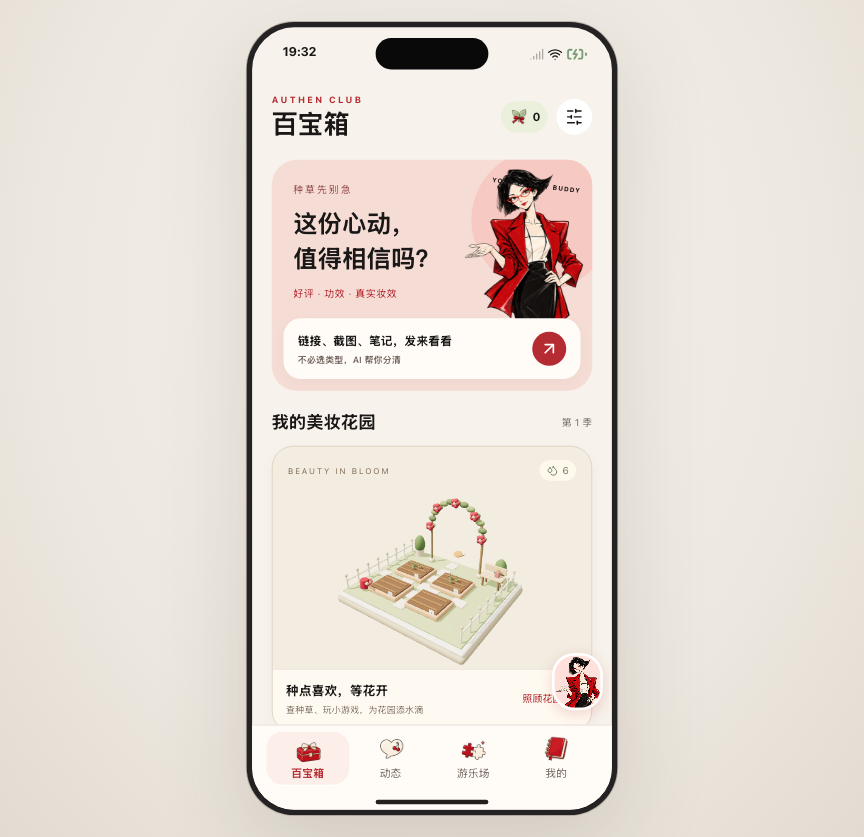
\includegraphics[width=0.82\textwidth]{../homepage/before/home-before.png}
\caption*{修改前：hero 下方直接进入「我的美妆花园」，无场景入口}
\end{minipage}\hfill
\begin{minipage}{0.48\textwidth}
\centering
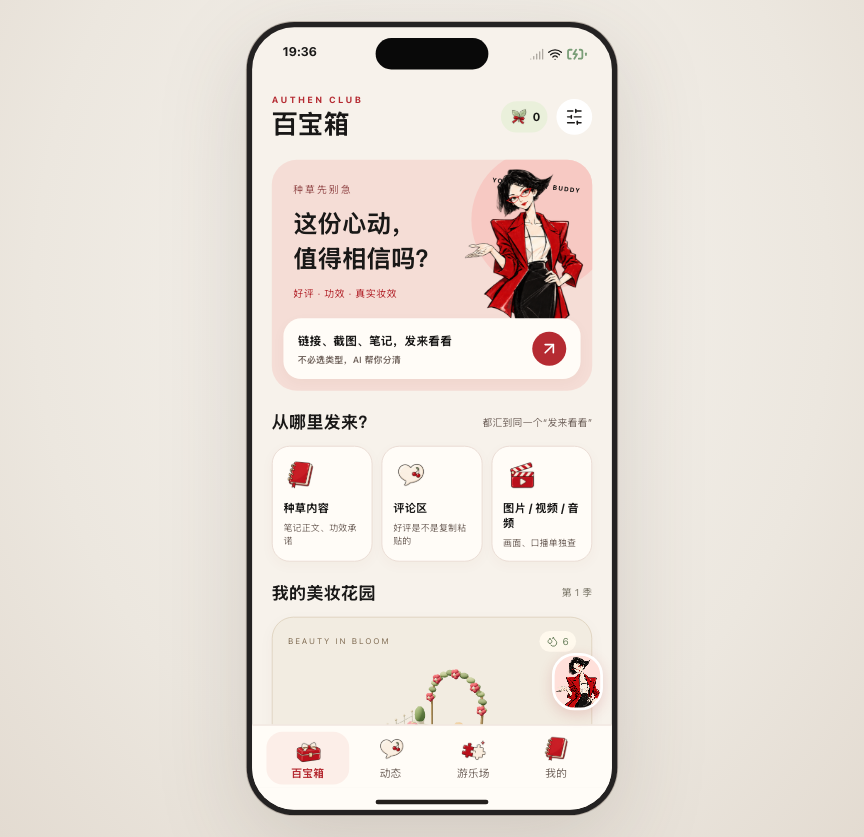
\includegraphics[width=0.82\textwidth]{../homepage/after/home-after.png}
\caption*{修改后：hero 下方新增「从哪里发来？」三张场景卡}
\end{minipage}
\end{figure}

\begin{figure}[h]
\centering
\begin{minipage}{0.31\textwidth}
\centering
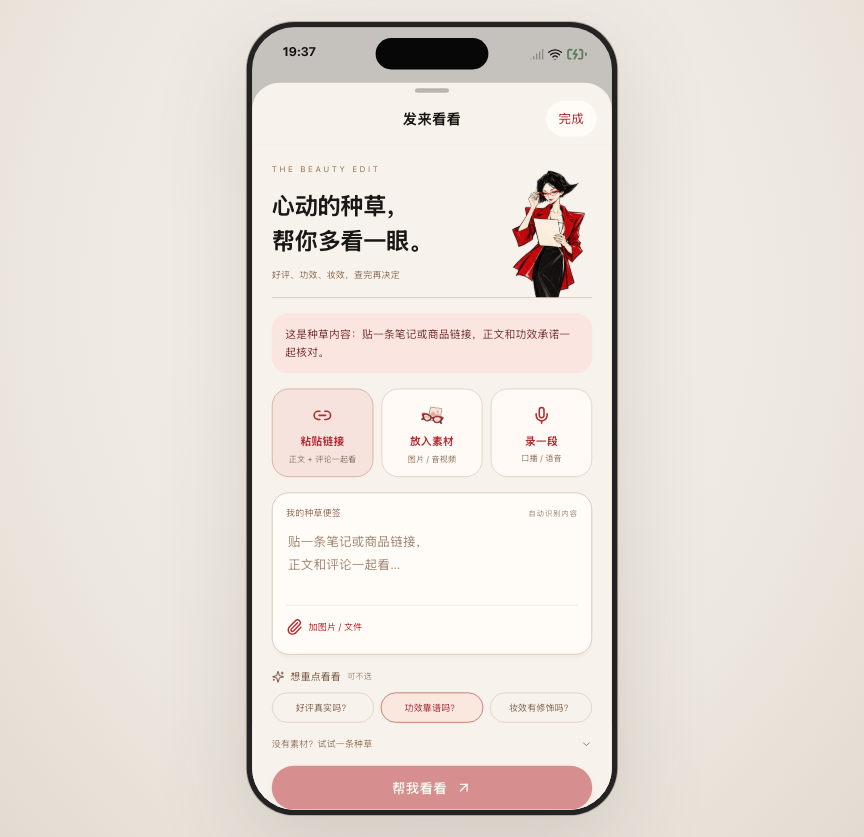
\includegraphics[width=0.9\textwidth]{../homepage/after/scenario-note.png}
\caption*{种草内容场景}
\end{minipage}\hfill
\begin{minipage}{0.31\textwidth}
\centering
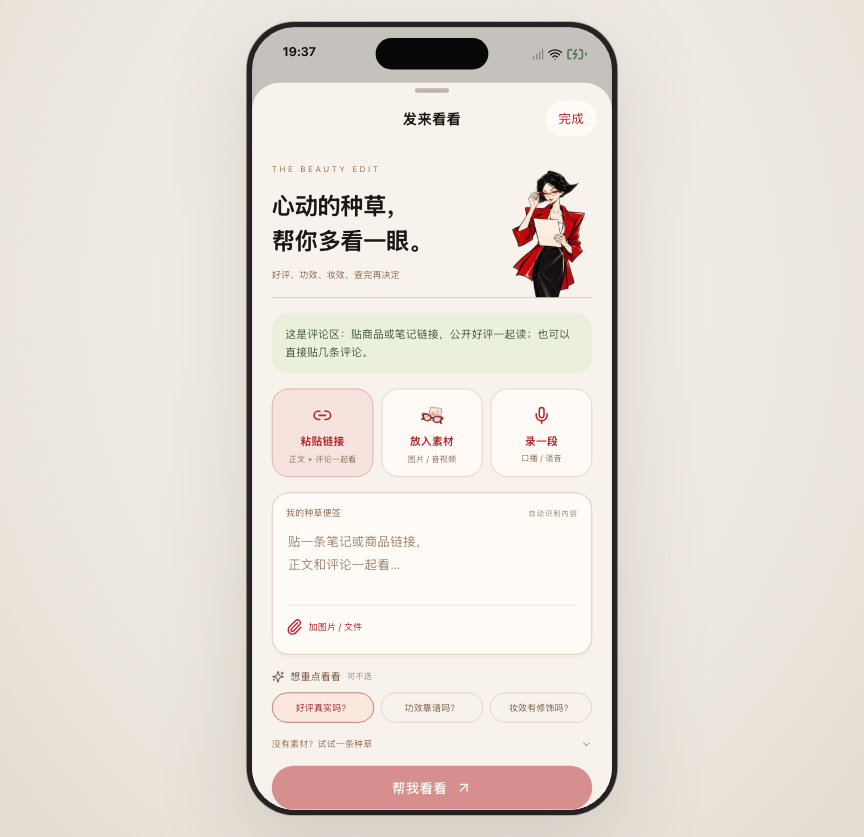
\includegraphics[width=0.9\textwidth]{../homepage/after/scenario-comments.png}
\caption*{评论区场景}
\end{minipage}\hfill
\begin{minipage}{0.31\textwidth}
\centering
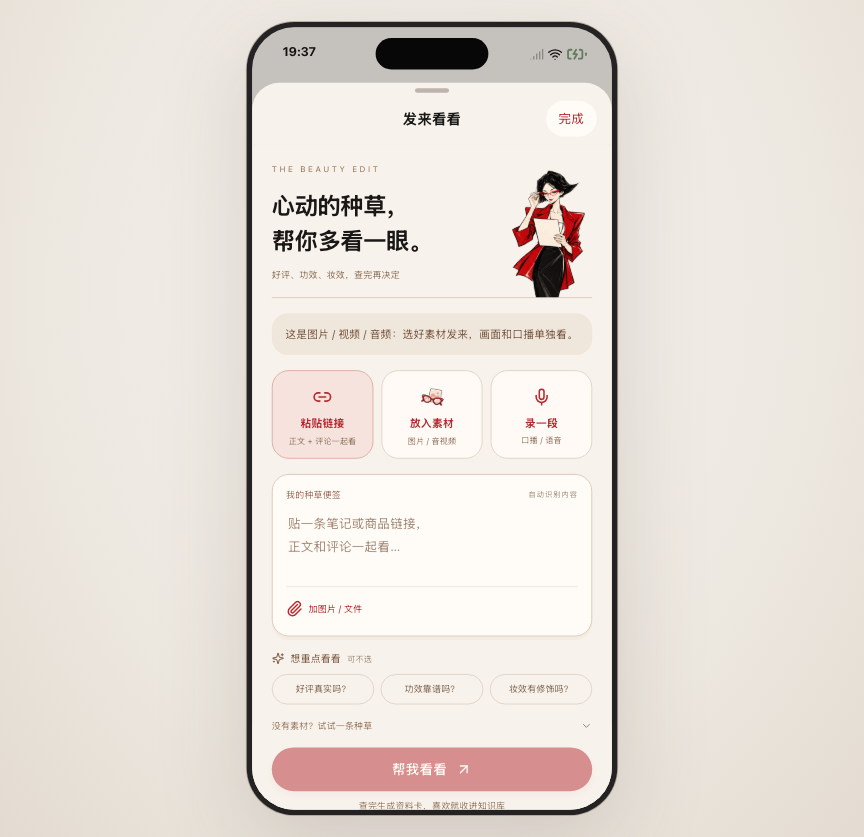
\includegraphics[width=0.9\textwidth]{../homepage/after/scenario-media.png}
\caption*{图片/视频/音频场景}
\end{minipage}
\end{figure}

\begin{figure}[h]
\centering
\begin{minipage}{0.48\textwidth}
\centering
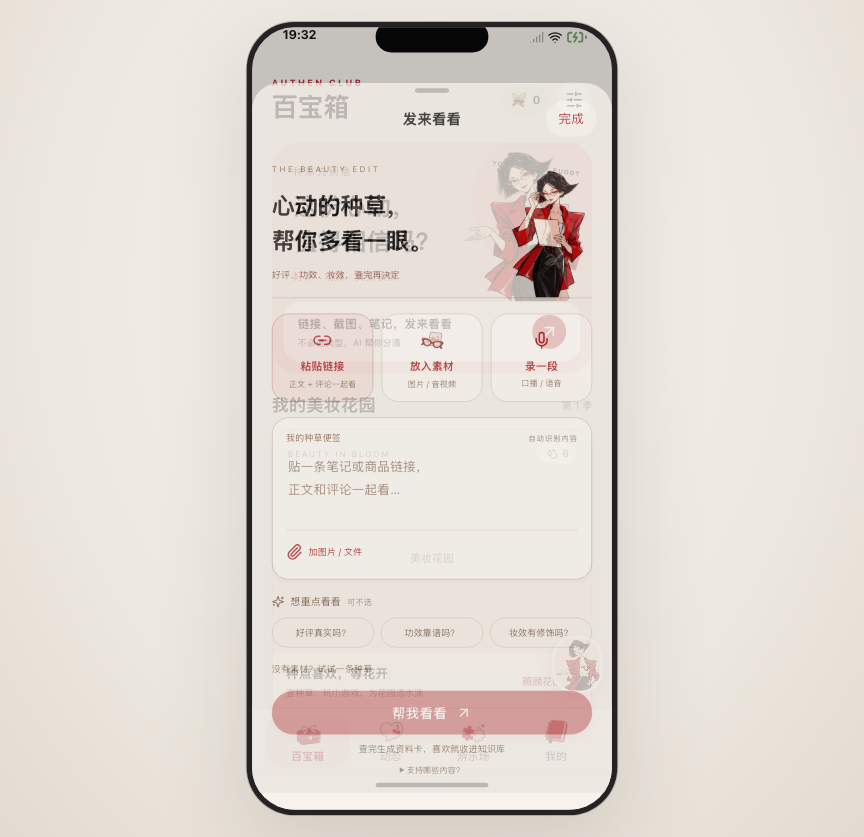
\includegraphics[width=0.82\textwidth]{../homepage/before/smart-sheet-before.png}
\caption*{修改前原「发来看看」弹窗}
\end{minipage}\hfill
\begin{minipage}{0.48\textwidth}
\centering
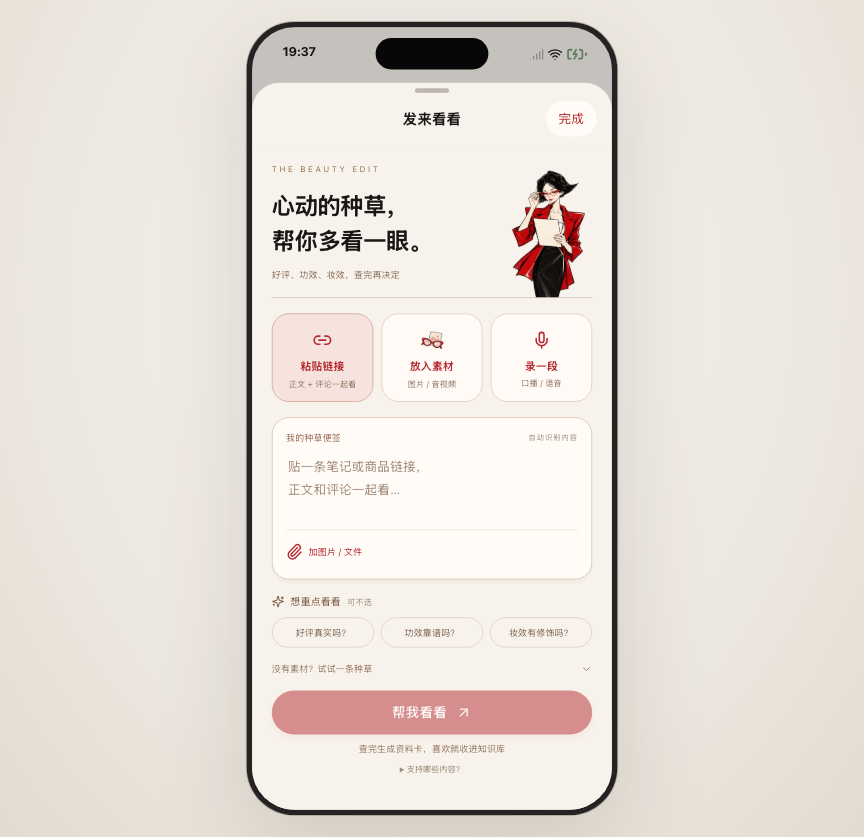
\includegraphics[width=0.82\textwidth]{../homepage/after/smart-sheet-after.png}
\caption*{hero 主入口回归：无场景引导条，原流程不变}
\end{minipage}
\end{figure}

% ===================== 11 =====================
\section{复现指南与交付清单}

\subsection{复现步骤}
\begin{enumerate}[label=\arabic*.]
\item 启动本地消费者端后端（shard\_02 改用独立端口 4192），命令见各分片 RUNBOOK。
\item 按分片 RUNBOOK（已留存于足迹 batch\_logs）执行批次脚本。
\item 运行合并复算脚本生成汇总；统计以 \texttt{summary\_140.json} 为准，脚本见 \texttt{scripts/}。
\end{enumerate}

\subsection{交付文件清单（根目录 QA-140-report/）}
\begin{itemize}
\item \texttt{data/merged\_140.jsonl}：140 条合并明细（结构化全字段）。
\item \texttt{data/merged\_140.csv}：140 条扁平表（UTF-8-BOM）。
\item \texttt{data/summary\_140.json}：独立复算汇总（通过数、多维分布、混淆矩阵、失败类型、源文件 sha256）。
\item \texttt{data/failures\_123.json}：123 条未通过清单。
\item \texttt{footprint/}：逐样本 request/response/run.log + 批次日志/脚本/运行说明 + index.csv。
\item \texttt{figures/}：7 张统计图表 PNG。
\item \texttt{homepage/}：修改说明、前后截图、源码变更包 zip、统一 diff、测试/构建日志。
\item \texttt{report/report.tex} 与 \texttt{report/report.pdf}：本报告源码与实际编译 PDF。
\item \texttt{scripts/}：合并复算、足迹组装、出图脚本（可重跑）。
\end{itemize}

\end{document}
